% RQ2
\newpage
\section{Performance prediction}
\label{sec:performanceprediction}
In this section, the results given by the empirical study (\autoref{sec:empiricalstudy}) will be used for predicting performance on unseen new datasets, in order to answer the second research question: \textit{Is it possible to create an extensive data profile to estimate performance on unseen datasets?}
~\\~\\Performance prediction aims to estimate the performance scores of an error detection strategy, on a specific dataset, without having to run the strategy beforehand or having the clean dataset at hand. The dataflow/workflow of this process is shown in \autoref{fig:method_estimation}.
When estimators are capable of estimating the performance scores, one could use this estimation to choose an error detection strategy. This contributes to the main research question of choosing a fitting error detection algorithm for a specific relational dataset.

To make predictions on the performance scores, information about the dataset is extracted beforehand, called a dataset profile. This profile contains high-level information that is of low cost computationally. This high-level information will most presumably give an idea on how to fix the errors inside the dataset, which could be input to predict the performance score a specific error detection strategy will get on that particular dataset. An estimator is then trained for each error detection strategy, with all the data profiles. The main notion is that error detection strategies assumably have comparable performance scores on similar datasets in terms of these high-level information profiles. 

\begin{figure}[h]
	\centering
	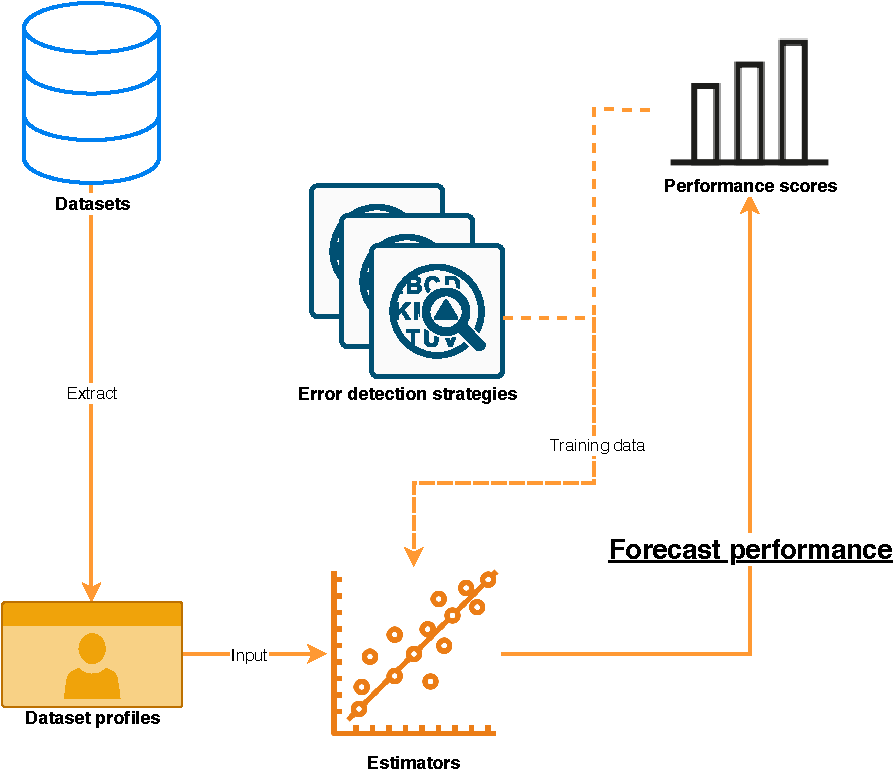
\includegraphics[width=0.9\textwidth]{thesis/Figures/Method/PerformanceEstimation-Profiler.pdf}
	\caption{Performance scores estimation}
	\label{fig:method_estimation}
\end{figure}

\newpage
\paragraph{Analogy} One can think of this like going into a car garage with a broken car. The garage employee will take a quick look at the outside of the car, at the brand of the car and will ask you some questions about the problems you have. This small \textit{\textbf{assessment}} could give an idea on what fixing strategy will most probably work best to fix the car. In his mind, the employee will have a list of strategies to fix a car (replace tyres, oil change, etc..) and will \textbf{\textit{estimate the possible outcomes}} (or performance) of those strategies (speed of fixing, longevity, cost, etc..), based on the performance of these strategies on previous cars with a similar assessment. Although in the execution, the results might differ from what the employee had in mind. The estimation might not give the exact performance outcome.

This is the same with the prediction of the performance scores of error detection strategies, as depicted in \autoref{fig:method_estimation}. An estimator, in this case a regression model, will look at a dataset and do the small assessment (\textbf{\textit{dataset profile}}), like looking at the car. From this small assessment, the estimator will try to \textbf{\textit{estimate the performance scores}} for each of the error detection strategies in mind based on previous datasets and the performance on those datasets, like the car garage employee guessed the outcome of replacing the tyres based on experience with previous cars. However, there will be a difference between the real outcome of that strategy (experimental results from \autoref{sec:empiricalstudy}) and the estimations of the performance scores. 

This idea was proposed by \cite{Mahdavi2019-pk}. This paper proposes the idea of a 'dirtiness profile'. The idea is that error detection tools would have similar performance on similar datasets. Regression models would be trained and tested on characteristics of the dataset, also called 'dirtiness profile' (input) and F1-scores (output). The following section will be a modification of the research by \cite{Mahdavi2019-pk}. 
The goal will be to estimate performance and predict values as close to the real performance scores as possible, which can be measured with the mean squared error.
The train and test in and outputs are retrieved from the empirical study (\autoref{sec:empiricalstudy}). One main difference is that this research will solely focus on automated prediction, where no rules or patterns from the ground truth are taken, and no user-defined configurations need to be created in order to perform the predictions. Besides, multiple new input features will be introduced to see if the performance can be increased. Lastly, instead of directly estimating the F1-score, as done by \cite{Mahdavi2019-pk}, estimators will be trained on both the recall and precision scores. The F1-score can be calculated using both estimated scores.
A regression model is trained for every strategy (error tool and specific configuration, see \autoref{fig:eachstrategy}). 

\begin{figure}[h]
	\centering
	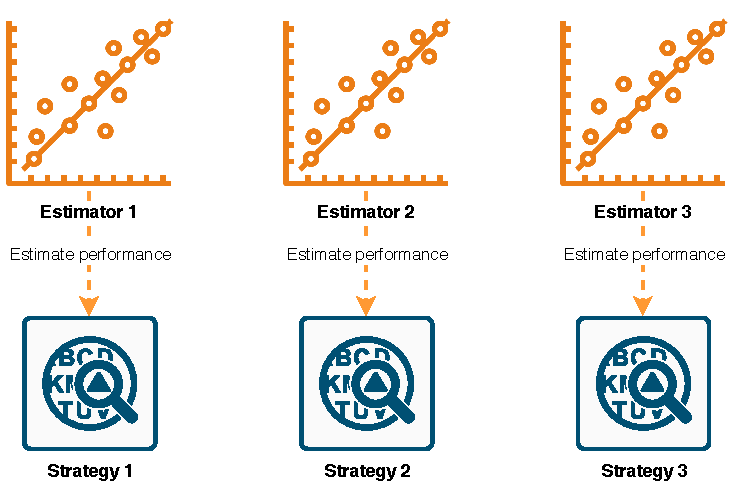
\includegraphics[width=0.8\textwidth]{thesis/Figures/Method/PerformanceEstimation-OnlyEstimate.pdf}
	\caption{Each strategy will result in a separate estimator}
	\label{fig:eachstrategy}
\end{figure}

\subsection{Data profiles}
\label{subsec:dataprofiles}
This section will discuss the methodology of creating a data profile for a dataset, to elaborate the first part of the second research question: \textit{Is  it  possible  to  \textbf{create an extensive data profile} to estimate performance on unseen datasets?}
~\\~\\The data profiles are created using only top-level features, without having any previous knowledge about the datasets. In this research, the focus lies only on features that are extractable without knowing the ground truth, only the dirty dataset. The basic set of features used is a subset of the proposed features from \cite{Mahdavi2019-pk}. However, all features where some information about the ground truth was necessary (rules, patterns or other heuristics found in the clean dataset), were left out. The features are extracted from each column. Then, aggregates of these column-wise extracted features are aggregated using the mean, variance, min and max to get a representation of feature distributions for each column in a dataset, with homogeneous output in size for training the regression models later on. These aggregated features representing the dataset profiles are the input values for the estimators. 

\begin{table}[H]
\centering
\begin{adjustbox}{center}
	\begin{tabular}{lll}
		Feature                   & Type       & Description \\ \hline
		characters\_unique        & characters & The number of unique characters \\
		characters\_alphabet      & characters & The number of only alphabetical characters \\
		characters\_numeric       & characters & The number of only numerical characters \\
		characters\_punctuation   & characters & The number of punctuation characters \\
		characters\_miscellaneous & characters & The number of characters not included in the categories above \\
		words\_unique             & words      & The number of unique words \\
		words\_alphabet           & words      & The number of fully alphabetical words \\
		words\_numeric            & words      & The number of fully numerical words (decimals included) \\
		words\_punctuation        & words      & The number of characters used solely as punctuation \\
		words\_miscellaneous      & words      & The number of words not included in the categories above  \\
		words\_length             & words      & The average word length \\
		cells\_unique             & cells      & The number of unique cells \\
		cells\_alphabet           & cells      & The number of completely alphabetical cells \\
		cells\_numeric            & cells      & The number of fully numerical cells (decimals included) \\
		cells\_punctuation        & cells      & The number of cells with only punctuation characters \\
		cells\_miscellaneous      & cells      & The number of cells not included in the categories above\\
		cells\_length             & cells      & The total length of cells combined \\
		cells\_null               & cells      &  The number of empty cells 
	\end{tabular}
	\end{adjustbox}
	\caption{All column-wise extracted features for the dataset profiles}
	\label{tab:profilefeatures}
\end{table}

\subsection{Experimental setup}
%%% Leave-one-out training
% Real performance dataframe
% Estimation performance dataframe
% Calculate errors
This section will describe the experiments to test the estimation capabilities of possible estimators, to answer the other part of the second research question: \textit{Is it \textbf{possible} to create an extensive data profile \textbf{to estimate performance} on unseen datasets?}
~\\~\\To discover whether the discussed data profiles are useful in estimating the performance of error detection tools, the setup from \autoref{sec:empiricalstudy} is updated. \autoref{fig:method_estimation} shows the flow of estimating the performance scores of the run error detection tools on the datasets. The goal of this workflow is to estimate the performance scores of error detection strategies on unseen datasets.

The estimators will be created as scikit-learn (\cite{Pedregosa2011-su}) pipelines. Not only does this allow interchangeable regression models, but also configurable data preparation. The different configurable parts all have certain assumptions. A combination of all possible settings will be created and tested in order to find the best configuration possible.

To evaluate the estimators and find the best configuration for the estimators, an experiment has to be conducted to evaluate the prediction potential of these estimators.
In reality, the estimators will be trained on all available training datasets and used to estimate performance scores on unseen datasets. However, with unseen datasets, only the dirty dataset is available, not the clean dataset. This means that it is not possible to evaluate the prediction capabilities of these estimators in a straight-forward way.
\textbf{Leave-one-out cross-validation} is a method to simulate the behaviour of training on as many training datasets as possible, while still being able to evaluate the results afterwards, by leaving only one dataset out of that training set at the time. \autoref{tab:leave-one-out} shows such an example for leave-one-out training with 4 datasets available. In each iteration, a single dataset is left out of the training set, simulating the performance prediction for the left out dataset. This will result in a performance score prediction $\hat{y}(s_i, d_j)$ for a certain strategy $s_i$ and dataset $d_j$. 

 \begin{table}[H]
\centering
\begin{tabular}{|l|l|l|l|l|l|}
\cline{1-4} \cline{6-6}
\textbf{$d_1$} & \textbf{$d_2$} & \textbf{$d_3$} & \textbf{$d_4$} &                 & \textbf{Output} \\ \cline{1-4} \cline{6-6} 
\textit{Estimate}          & Train         & Train         & Train         & $\rightarrow$ & $\hat{y}(s_i, d_1)$      \\ \cline{1-4} \cline{6-6} 
Train         & \textit{Estimate}          & Train         & Train         & $\rightarrow$ & $\hat{y}(s_i, d_2)$      \\ \cline{1-4} \cline{6-6} 
Test          & Train         & \textit{Estimate}          & Train         & $\rightarrow$ & $\hat{y}(s_i, d_3)$     \\ \cline{1-4} \cline{6-6} 
Test          & Train         & Train         & \textit{Estimate}          & $\rightarrow$ & $\hat{y}(s_i, d_4)$      \\ \cline{1-4} \cline{6-6} 
\end{tabular}
\caption{Leave one out training example for a strategy $s_i$ and datasets $d_{1-4}$}
\label{tab:leave-one-out}
\end{table}

For each dataset $d$ from $D$ datasets and error detection strategy $s$ from all strategies $S$, the leave-one-out evaluation as described above and in \autoref{tab:leave-one-out} will be executed. This will leave a $m \times n$ matrix of estimated performance scores as shown in \autoref{tab:estimatedscores}, representing a $m$ strategies and the $n$ available datasets.
For comparison, the real scores that are obtained from the empirical study from \autoref{sec:empiricalstudy} are shown in the same format in \autoref{tab:realscores}.

 \begin{table}[h]
	\centering
	\addtolength{\leftskip} {-2cm}
	\addtolength{\rightskip}{-2cm}
	\captionsetup[subtable]{position = below}
	\captionsetup[table]{position=top}
	\caption{$m \times n$ (strategies $\times$ datasets) matrix of scores}
		\begin{subtable}{0.5\linewidth}
		\centering
		\begin{tabular}{|l|l|l|l|l|}
			\hline
			               & \textbf{$d_1$}      & \textbf{$d_2$}      & \textbf{...} & \textbf{$d_n$}      \\ \hline
			\textbf{$s_1$} & $\hat{y}(s_1, d_1)$ & $\hat{y}(s_1, d_2)$ & ...          & $\hat{y}(s_1, d_n)$ \\ \hline
			\textbf{$s_2$} & $\hat{y}(s_2, d_1)$ & $\hat{y}(s_2, d_2)$ & ...          & $\hat{y}(s_2, d_n)$ \\ \hline
			\textbf{...}   & ...                 & ...                 & ...          & ...                 \\ \hline
			\textbf{$s_m$} & $\hat{y}(s_m, d_1)$ & $\hat{y}(s_m, d_2)$ & ...          & $\hat{y}(s_m, d_n)$ \\ \hline
		\end{tabular}
		\caption{Estimated performance scores}
		\label{tab:estimatedscores}
	\end{subtable}
	\hspace*{4em}
	\begin{subtable}{0.5\linewidth}
		\centering
		\begin{tabular}{|l|l|l|l|l|}
			\hline
			               & \textbf{$d_1$} & \textbf{$d_2$} & \textbf{...} & \textbf{$d_n$} \\ \hline
			\textbf{$s_1$} & $y(s_1, d_1)$  & $y(s_1, d_2)$  & ...          & $y(s_1, d_n)$  \\ \hline
			\textbf{$s_2$} & $y(s_2, d_1)$  & $y(s_2, d_2)$  & ...          & $y(s_2, d_n)$  \\ \hline
			\textbf{...}   & ...            & ...            & ...          & ...            \\ \hline
			\textbf{$s_m$} & $y(s_m, d_1)$  & $y(s_m, d_2)$  & ...          & $y(s_m, d_n)$  \\ \hline
		\end{tabular}
		\caption{Real performance scores}
		\label{tab:realscores}
	\end{subtable}%
\end{table}
       

To assess the estimated performance scores as shown in \autoref{tab:estimatedscores}, the scores will be compared element-wise with the real performance scores shown in \autoref{tab:realscores}. To do so, the difference between the estimation of the score and the score itself will be calculated. This is the \textbf{estimation error}. 
The real score is denoted as $y$, which is a performance score result of the empirical study, for example precision, recall or f1-score. The estimated score is denoted as $\hat{y}$. The error for a single score, for a specific error detection strategy and dataset is the following:

\begin{equation}
	e(s, d) = \hat{y}(s, d) - y(s, d)
\end{equation}

To quantify the ability of an estimator pipeline to estimate the real performance scores of error detection strategies, the mean squared error for all the (strategy, dataset) tuples is taken. 

\begin{equation}
	MSE = \frac{1}{|D||S|} \sum_{d \in D} \sum_{s \in S} e(s, d)^2
\end{equation}

This mean squared error will give a method of comparison between different estimator configurations. For the best estimator configuration, the estimation error distribution will be shown to find how the estimator generally performs, for example by comparing the number of over- and under-estimations.

\subsection{Estimator selection}
\label{subsec:estimatorselection}
% Regression model selection
Now that a score for comparing estimators has been covered, the range of estimator configurations will be discussed.
The estimator pipeline consists of four possible parts:
\begin{enumerate}
	\item Feature normalization
	\item Feature selection
	\item Principal component analysis
	\item Regression model
\end{enumerate}

Each part of the pipeline is configurable. The first three parts can be left out, leaving only a regression model with the normal dataset profile as input. 

\subsubsection{Feature normalization or standardization}
The three chosen possibilities for feature normalization are:
\begin{itemize}
	\item None: No normalization or scaling is applied.
	\item StandardScaler (\verb|sklearn.preprocessing.StandardScaler|): Standardize features by removing the mean and scaling to unit variance. The scaler will be trained on the training sample so that after the training, each feature can be scaled using the distributions of the training set.
	\item Normalizer (\verb|sklearn.preprocessing.Normalizer|): Normalize samples individually to unit norm. Each sample (i.e., each row of the data matrix) with at least one non zero component is rescaled independently of other samples so that its norm equals one. It is executed with a default $l_2$-norm
\end{itemize}

\subsubsection{Feature selection}
For feature selection, different trainable configurations are possible to optimize the number of input dimensions for the later parts of the pipeline. Research has shown that using too many input features for machine learning will decrease performance (\cite{Trunk1979-sq}). To circumvent the curse of dimensionality, feature selection methods can be put in the machine learning pipeline to learn which features to use as well. 

\begin{itemize}
	\item None: No dimensionality reduction is applied in the pipeline.
	\item Variance Threshold (\verb|sklearn.feature_selection.VarianceThreshold|): This removes all features that have a variance below a certain threshold in the training dataset. The threshold has to be set to some value.
	\item Select From Model (\verb|sklearn.feature_selection.SelectFromModel|): It selects the features based upon the importance weights of the trained regressor. On default, all features that have a weight above the mean of all feature weights are selected.
	\item Select K Best (\verb|sklearn.feature_selection.SelectKBest|): This method selects the K best features according to a specified score. In this case, the \\\verb|sklearn.feature_selection.f_regression| method is used, where the correlation between the target values and each separate (univariate) feature is calculated.
\end{itemize}

Besides feature selection methods that are used directly in the machine learning pipeline, feature selection can also be done in retrospect, which will be discussed in \autoref{subsec:featureselection}.

\subsubsection{Principal component analysis}
Principal component analysis is a dimensionality reduction method invented over a century ago (\cite{Pearson1901-de}), but still has a strong use case in machine learning today. As said in the previous section, too many input features will lead to worse performance with the small number of input samples to train. A linear PCA will reduce the whole feature space to N number of components holding the most variance for all the input points. To transform and capture non-linear relations, also Kernel PCA will be used. This will be useful, as most regression models will not be capable of distinguishing between non-linear relations.

\begin{itemize}
	\item None: No dimensionality reduction using PCA will be done.
	\item PCA (\verb|sklearn.decomposition.PCA|): Linear dimensionality reduction using Singular Value Decomposition of the data to project it to a lower-dimensional space. Highly sensitive to scaling of the features (recommended to scale beforehand).
	\item Kernel PCA (\verb|sklearn.decomposition.KernelPCA|): Allows for non-linear dimensionality reduction through using specified kernels. An RBF (radial basis function) kernel is commonly used for projecting non-linear relation onto a linear separable projection.
\end{itemize}

\subsubsection{Regression model}
As the final step in the pipeline, a regression model is present. It takes in the input features from the last step in the pipeline, depending on which normalization, feature selection and/or principal component analysis methods are chosen. The regression model will take the transformed data profile inputs from all the training datasets and tries to estimate the selected real scores. This score always will be between 0 and 1, inclusive. So at the end of each estimator, a limiter will be put into place not to have any impossible scores. The possible regression models are stated below. All models have certain assumptions that the workings build upon. 

\begin{itemize}
	\item Linear Regression (\verb|sklearn.linear_model.LinearRegression|): This regression model fits a linear model that minimizes the sum of errors between the observed estimation and real observations. This method can be sensitive to outliers, due to its reliance on the square of errors.
	\item K-nearest Neighbors Regression (\verb|sklearn.neighbors.KNeighborsRegressor|): The output is estimated by comparing it to the nearest neighbors in the training samples. The K nearest points are weighted equally and the training scores will be combined as an estimation.
	\item Ridge Regression (\verb|sklearn.linear_model.Ridge|): This model solves a regression model where the loss function is the linear least squares function and regularization is given by the $l_2$-norm
	\item Bayesian Ridge Regression (\verb|sklearn.linear_model.BayesianRidge|): This model can be used for estimating the regularization parameters as well, the regularization parameter is not set in a hard sense but tuned to the data at hand. It then estimates the ridge regression model.
	\item Decision Tree Regression (\verb|sklearn.tree.DecisionTreeRegressor|): This is a regression model that outputs different discrete output levels based on an outcome of a decision tree, comparing individual features to certain learned values.
	\item Support Vector Regression (\verb|sklearn.svm.SVR|): A support vector machine-based regression model. Like normal Support Vector Classification, the regression model depends only on a subset of the training data, making it more robust against outliers.
	\item Gradient Boosting Regression (\verb|sklearn.ensemble.GradientBoostingRegressor|): Produces a predictive model from an ensemble of weak predictive models. In each stage, a regression tree is fit on the negative gradient of the least squares regression loss.
	\item AdaBoost Regression (\verb|sklearn.ensemble.AdaBoostRegressor|): A meta-estimator that trains multiple regression models (default \verb|DecisionTreeRegressor|) and consequently adjusts weights of input samples depending on the error of the previous estimator.
	\item Multi-layer Perceptron Regression (\verb|sklearn.neural_network.MLPRegressor|): A neural network-based regression model. Capable of capturing non-linear relations, however, that would require multiple layers, which will, on its turn, require more training samples. 
\end{itemize}

\subsection{Combination of estimators}
% Separate precision & recall estimator
% Combined values
Now that all the components for the estimator have been described, one can try to create ensemble estimators. In the study of \cite{Mahdavi2019-pk}, the F1-score was directly estimated. Knowing that this metric is directly built from both the precision and recall, it intuitively makes sense to first create estimators for the precision and recall (two separate estimator configurations), and use the output of these two configurations in combination to estimate the F1-score. Therefore, besides only calculating the MSE for an F1-score estimator, it will be compared to the MSE of the ensemble F1-score estimator.

\subsection{Evaluation}
\label{subsec:evaluation_performanceprediction}
To evaluate the experiment results as discussed above, the results will be both qualitatively and quantitatively analyzed to find an answer the research question: \textit{Is it possible to create an extensive data profile to estimate performance on unseen datasets?};

\paragraph{Qualitative} First, the best estimator configuration will be chosen according to the lowest mean squared error of the estimations of real performance scores. This chosen estimator configuration will be qualitatively judged on the distribution of estimation errors. To deem the estimation of performance successful, the error distribution should be heavily centered around 0, indicating that most estimations are close to perfect. Also, the distribution should not be uniform (which will indicate random errors) and should not have clusters of outliers, which indicate underestimations or overestimations. 

\paragraph{Quantitative} Second, to add more substance to the evaluation, a baseline estimator method will be executed to see if the selected estimator has an improvement over that baseline method. The baseline estimator will be simply taking the average of the performance scores achieved on the training datasets. Only taking the average of the input performance scores is similar to regression without any weights to the input variables.
An example is shown in \autoref{tab:method_baseline_estimation} where the baseline estimators "trains" on $d_1$ and $d_2$. The estimation of a new dataset $d_3$ will be the average of the already known dataset performance scores, namely the average of 1 and $0.2$, which is $0.6$.
\\If the estimators improve over this baseline method in terms of mean squared error, median absolute error and mean absolute error, it shows that the estimator is capable of learning information from the dataset profiles and giving a useful estimation, better than the baseline.

\begin{table}[]
\centering
\begin{tabular}{l|lll}
           & $d_1$ (Train) & $d_2$ (Train) & $d_3$ (Test) \\ \hline
F1         & 1             & 0.2             & ?            \\
Estimation & -             & -             & \textbf{0.6}
\end{tabular}
\caption{Example baseline performance estimation for some example strategy $s$}
\label{tab:method_baseline_estimation}
\end{table}

~\\If the assessments are both qualitatively and quantitatively positive, it can be deemed possible to create an extensive data profile to estimate performance on unseen datasets.